\documentclass[12pt, twoside]{article}
\input{../preamble}

\fancyhead[LO]{La Scuola d'Italia / Dr.\ Huson / IB Math: Practice \\* 1 May 2026}
\fancyhead[RO]{\fbox{\begin{minipage}{6cm}\footnotesize First \& Last name:\\[0.5cm]\end{minipage}}}
\fancyfoot[C]{\thepage}

\begin{document}
\subsubsection*{11.15 Do Now: Introduction to Periodic Functions (no calculator)}

The graphs of $\sin$ and $\cos$ can be stretched, shifted, and translated to model
periodic phenomena (tides, springs, rotating wheels). The general form is
$$f(x) = a\,\sin\!\bigl(b(x + c)\bigr) + d \qquad \text{or} \qquad f(x) = a\,\cos\!\bigl(b(x + c)\bigr) + d,$$
where each of $a$, $b$, $c$, $d$ controls one feature of the graph:
\begin{center}
\begin{tabular}{l l l}
$|a|$ & amplitude & half of $(\max - \min)$; vertical stretch \\
$b$   & frequency factor & period $T = \dfrac{2\pi}{b}$ \\
$c$   & phase shift      & horizontal translation by $-c$ \\
$d$   & vertical shift   & midline $y = d$ \\
\end{tabular}
\end{center}

\textbf{Example.} \quad $f(x) = 2\sin\!\left(\dfrac{\pi}{2}(x - 1)\right) + 3$ has
$a = 2$, $b = \dfrac{\pi}{2}$, $c = -1$, $d = 3$, period $T = 4$.
\vspace{0.7cm}

\begin{center}
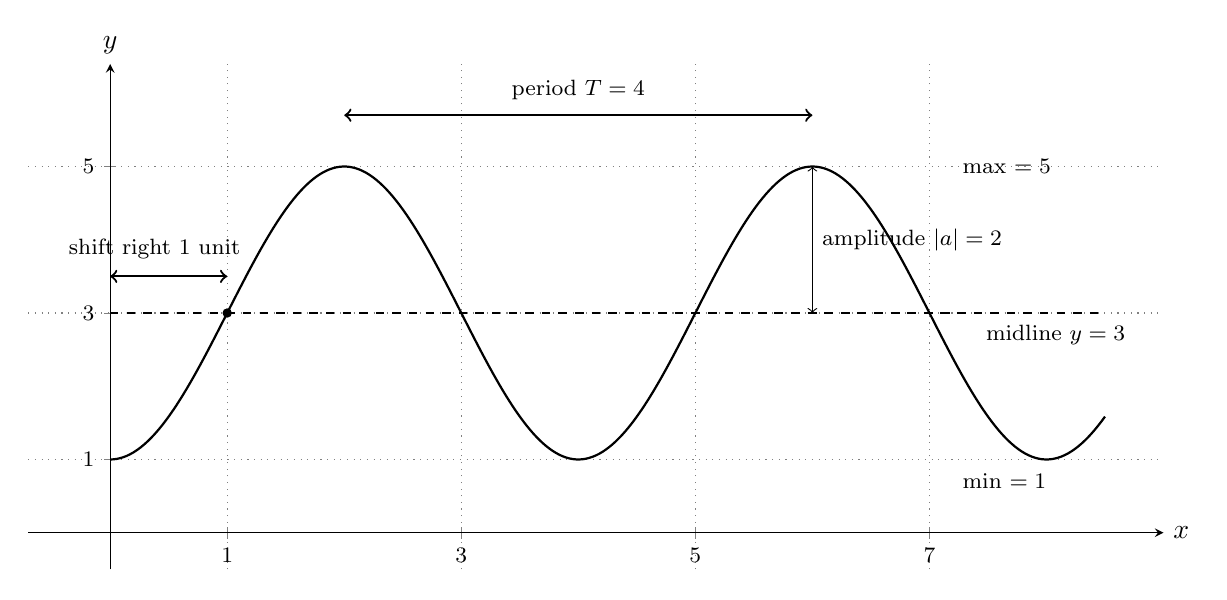
\begin{tikzpicture}
\begin{axis}[
    width=16cm, height=8cm,
    axis lines=middle,
    xlabel={$x$}, ylabel={$y$},
    xlabel style={at={(ticklabel* cs:1)}, anchor=west},
    ylabel style={at={(ticklabel* cs:1)}, anchor=south},
    xmin=-0.7, xmax=9,
    ymin=-0.5, ymax=6.4,
    xtick={1, 3, 5, 7},
    ytick={1, 3, 5},
    grid=major, grid style={dotted, gray},
    samples=300,
    tick label style={font=\footnotesize},
]
\addplot[thick, domain=0:8.5] {2*sin(deg((pi/2)*(x - 1))) + 3};
% midline
\addplot[dashed, thin, domain=0:8.5] {3};
\node[anchor=west, font=\footnotesize] at (axis cs:7.4,2.7) {midline $y = 3$};
\node[anchor=west, font=\footnotesize] at (axis cs:7.2,5) {max $= 5$};
\node[anchor=west, font=\footnotesize] at (axis cs:7.2,.7) {min $= 1$};
% Period bracket peak-to-peak (x=2 to x=6)
\draw[<->, thick] (axis cs:2,5.7) -- (axis cs:6,5.7);
\node[font=\footnotesize] at (axis cs:4,6.05) {period $T = 4$};
% Amplitude bracket at the right side
\draw[<->] (axis cs:6,3) -- (axis cs:6,5);
\node[anchor=west, font=\footnotesize] at (axis cs:6,4) {amplitude $|a| = 2$};
% Phase shift arrow from y-axis to just above (1, 3)
\draw[<->, thick] (axis cs:0,3.5) -- (axis cs:1,3.5);
\node[circle, fill=black, inner sep=1.2pt] at (axis cs:1,3) {};
\node[anchor=south, font=\footnotesize] at (axis cs:0.38,3.6) {shift right 1 unit};
\end{axis}
\end{tikzpicture}
\end{center}
\vspace{0.7cm}

\textbf{Reading $a$, $b$, $c$, $d$ from a graph (inverse problem).}
\begin{itemize}[itemsep=0cm, topsep=0.05cm]
\item $a = \dfrac{\max - \min}{2}$ (amplitude); \quad $d = \dfrac{\max + \min}{2}$ (midline)
\item $b = \dfrac{2\pi}{T}$, where $T$ is the period (peak-to-peak distance)
\item $c$ from a known point on the graph --- often a maximum, minimum, or zero crossing
\end{itemize}

\textit{Notation note.} Some IB problems write $f(x) = a\sin\!\bigl(b(x - c)\bigr) + d$ with a minus sign. The amplitude, period, and midline are unchanged; only the sign of $c$ flips.

\newpage

\textbf{Practice.}

\begin{enumerate}[itemsep=0.2cm]

%--- Problem 1: state amplitude / period / midline / max ---
\item For the function $f(x) = 3\sin(2x) - 1$, write down:
\begin{enumerate}[itemsep=0.5cm]
  \item[(a)] the amplitude;
  \item[(b)] the period;
  \item[(c)] the equation of the midline;
  \item[(d)] the maximum value of $f$.
\end{enumerate}


%--- Problem 2: cos with phase shift, find max location ---
\item For the function $g(x) = 4\cos\!\left(\dfrac{\pi}{6}(x - 2)\right) + 5$, find:
\begin{enumerate}[itemsep=0.5cm]
  \item[(a)] the amplitude;
  \item[(b)] the period;
  \item[(c)] the equation of the midline;
  \item[(d)] the smallest value of $x \ge 0$ at which $g$ is a maximum.
\end{enumerate}


%--- Problem 3: sketch with given axes ---
\item Sketch $y = 2\sin x + 1$ for $0 \le x \le 2\pi$. Mark the maximum value, minimum value, and the $y$-intercept.

\begin{center}
\begin{tikzpicture}
\begin{axis}[
    width=14cm, height=5.5 cm,
    axis lines=middle,
    xlabel={$x$}, ylabel={$y$},
    xlabel style={at={(ticklabel* cs:1)}, anchor=west},
    ylabel style={at={(ticklabel* cs:1)}, anchor=south},
    xmin=-0.3, xmax=7,
    ymin=-1.3, ymax=3.8,
    xtick={1.5708, 3.1416, 4.7124, 6.2832},
    xticklabels={$\pi/2$, $\pi$, $3\pi/2$, $2\pi$},
    ytick={-1, 1, 2, 3},
    minor y tick num=0,
    grid=major, grid style={dotted, gray!50},
    tick label style={font=\small},
]
\end{axis}
\end{tikzpicture}
\end{center}

%--- Problem 4: inverse problem from features ---
\item A function $f$ has the form $f(x) = a\sin\!\bigl(b(x + c)\bigr) + d$, with $a > 0$ and $b > 0$. The function has:
\begin{itemize}
  \item maximum value $7$ and minimum value $1$;
  \item period $8$;
  \item first maximum at $x = 1$.
\end{itemize}
Find the value of $a$, $b$, $c$, and $d$.

\end{enumerate}

\end{document}
